\subsection{Basalganglia} \label{subsec:basalganglien} \index{Basalganglia}
Die Basalganglia bestehen aus mehreren funktionell zusammengehörigen Kerngebieten im Marklager des Großhirns. Dazu zählen das \textbf{Striatum}, der \textbf{Globus pallidus}, der \textbf{Nucleus subthalamicus} \index{Nucleus! subthalamicus} und auch die \textbf{Substantia nigra} \index{Substantia nigra} des Mittelhirns. Das Striatum wiederum setzt sich aus dem \textbf{Nucleus caudatus}, dem \textbf{Putamen} und dem \textbf{Nucleus accumbens} zusammen. Gemeinsam bilden diese Kernstrukturen eine Funktionsschleife, die eine wichtige Rolle in der motorischen Regulation spielt \textsuperscript{\cite[Kap.~9]{trepel2011neuroanatomie}}. Der Großteil der eingehenden Information in dieses System stammt aus der Großhirnrinde und wird im Striatum in Empfang genommen. Von dort nehmen die Impulse entweder einen direkten oder indirekten Weg und verlässt die Basalganglia anschließend über den \textit{Globus pallidus interna} oder die \textit{Substantia nigra pars reticulata}. Diese Strukturen beeinflussen daraufhin Zentren, die an der Planung oder Ausführung bestimmter Bewegungen beteiligt sind. Dazu zählen Kerne im Thalamus, die wiederum zum den motorischen Arealen des Neocortex ziehen oder auch die Colliculi superiores \textsuperscript{\cite[Kap.~17]{paxinos2014rat}}.   

\subsubsection*{Striatum} \index{Striatum}
Das \textbf{Striatum} setzt sich beim Menschen aus dem \textbf{Ncl. caudatus} \index{Nucleus! caudatus}, \textbf{Putamen} \index{Putamen} und \textbf{Ncl. accumbens} \index{Nucleus! accumbens} zusammen (Abb.~\ref{fig:Nucleus_accumbens}, Abb.~\ref{fig:GP_CPu}). Dabei entwickelten sich der Ncl. caudatus und das Putamen aus einer gemeinsamen Kernanlage heraus und werden nur teilweise durch Fasern der Capsula interna voneinander getrennt. Der Ncl. caudatus legt sich c-förmig um das Putamen herum und besitzt dabei auf der einen Seite einen großen Kopf, der auf der anderen Seite in einen spitzen Schwanz übergeht. Auf der Kopfseite wird der Ncl. caudatus fast vollständig durch die Fasern der Capusula interna vom Putamen abgetrennt. Zur rostralen Seite hingegen kann man die Strukturen kaum voneinander abgrenzen. Der Nucleus caudatus bildet dabei über seine Ausdehnung hinweg die Seitenwand und Teile des Dachs des lateralen Ventrikels. Das Putamen liegt lateral zu der Capsula interna und dem Globus pallidus. Die dünne Faserschicht der \textit{Lamina medullaris lateralis} trennt das Putamen vom Globus pallidus ab. Lateral zum Putamen befindet sich weiße Substanz, in der eine dünne Lage graue Substanz eingebettet ist, die als Claustrum bezeichnet wird. Diese Struktur teilt die weiße Substanz in die Capsula externa und die Capsula extrema ein. Wiederum lateral zur Capsula extrema findet man den Cortex insularis (Inselrinde, Insula) \index{Insula} \textsuperscript{\cite[Kap.~14]{crossman2014neuroanatomy}, \cite[9]{trepel2011neuroanatomie}}. Bei der Ratte werden die Strukturen des Ncl. caudatus und des Putamen als Caudate-Putamen zusammengefasst.\\    
Das Striatum fungiert als primäre Inputstruktur der Basalganglia. Die Afferenzen stammen aus dem Cortex, der Substantia nigra und auch aus dem Ncl. centromedianus des Thalamus. Die Mehrheit dieser Axone besteht dabei aus den Fibrae corticostriatales, die aus fast allen Bereichen des Großhirns, besonders aber aus den motorischen, sensorischen und präfrontalen Arealen, stammen. Die Fasern entspringen den Pyramidenneuronen des Großhirns, die sich bevorzugt in der fünften und auch dritten  cortikalen Schicht aufhalten. Dabei existieren zwei unterschiedliche Typen dieser corticostriatalen Pyramidenneuron, basierend auf subcortikalen Kollateralen, die sie bilden. Die erste Gruppe wird als 'intertel-encepahlic' (IT) corticostriatales Neuron bezeichnet. Ihre Kollaterale befinden sich ausschließlich innerhalb des Striatum und dem Cortex. Die zweite Gruppe wird als 'pyramidal tract' (PT) corticostriatales Neuron klassifiziert. Sie liegen hauptsächlich im Frontallappen des Großhirns und bilden Projektionen zum Hirnstamm und zum Rückenmark als Fasern des Pyramidentrakts aus. Ihre Kollaterale ziehen dabei zum Striatum. All diese Neurone verwenden Glutamat als Neurotransmitter und haben damit einen erregenden Einfluss auf das Striatum \textsuperscript{\cite[Kap.~9]{trepel2011neuroanatomie}, \cite[17]{paxinos2014rat}}.\\
Das Striatum besteht zum Großteil aus nur einer Neuronenart, den \textbf{dornentragenden Projektionsneurone}, die inhibitorisches GABA als Neurotransmitter freisetzten. Sie machen etwa 95~\% der Zellmasse des Striatum aus und fungieren als Ziel eingehender Axone und gleichzeitig auch als ausgehende Projektionsfasern. Die übrigen Zellen des Striatum sind Interneurone. Basierend auf den Ort ihrer efferenten Fasern, lassen sich die dornentragenden Neurone in zwei gleichgroße Teilgruppen unterteilen. Die eine Teilgruppe projiziert zu den GABAergen Neuronen des Globus pallidus interna und der Substantia nigra pars reticulata. Dies ist Grundlage des 'direkten striatalen Projektionsweg', da unmittelbar monosynaptisch vom Striatum ausgehend auf die Output-Strukturen der Basalganglia verschaltet wird. Die andere Gruppe dornentragender Neurone bildet den 'indirekten striatalen Projektionsweg'. Sie senden ihre Axone ausschließlich zum Globus pallidus. Von dort projizieren Fasern weiter zum Globus pallidus interna, der Substantia nigra oder dem Ncl. subthalamicus. Damit wird die Information indirekt polysynaptisch zu den Ausgangszentren der Basalganglia geleitet \textsuperscript{\cite[Kap.~17]{paxinos2014rat}}. Das genaue Verschaltungsprinzip und die Funktion dieser Schleife wird später ausführlicher beschrieben. Zusammenfassend lässt sich sagen, dass über die corticostriatalen Fasern vorwiegend motorische Impulse das Striatum erreichen. Über die indirekten oder direkten Projektionen kann dieser Input entweder gefördert oder unterdrückt werden. Damit fungiert das Striatum als zentrale Schaltstelle motorischer Impulse. Seine Hauptaufgabe besteht dabei besonders in der integratorischen Beeinflussung dieser Impulse \textsuperscript{\cite[Kap.~9]{trepel2011neuroanatomie}}.\\  
\\ \noindent Im ventrorostalen Bereich des Striatums ist der Ncl. accumbens zu finden (Abb.~\ref{fig:Nucleus_accumbens}). Er zeigt, wie das restliche Striatum, ein ähnliches Verschaltungsprinzip. Zusätzlich erhält er allerdings auch Input aus der Amygdala und dem Hippocampus und bildet damit eine wichtiges Bindeglied zu limbischen System. Er fungiert dabei als Relaisstelle für die Verwirklichung von motivations- oder affektbedingtem Verhalten. Des Weiteren wird er auch mit dem Belohnungsystem und daraus resultierendem Suchtverhalten in Verbindung gebracht \textsuperscript{\cite[Kap.~14]{crossman2014neuroanatomy}}.  

\begin{figure}[H]
    \centering
    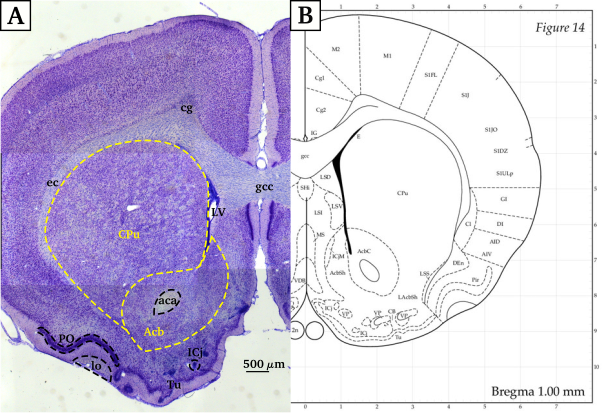
\includegraphics{pictures/Basalganglia/Nucleus_acumbens.png}
    \caption[Striatum]{\textbf{Striatum.} \textbf{A:} Das Striatum besteht aus dem Caudate putamen (CPu) und dem Ncl. accumbens (Acb). Um das Striatum herum sind folgende Strukturen zu sehen: anteriore Kommissur (aca), Cingulum (cg), Capsula externa (ec), Knie des Corpus callosum (gcc), Insula callejae (ICj), Tractus olfactorius lateralis (lo), lateraler Ventrikel (LV), primär olfaktorischer Cortex (PO), olfaktorisches Tubercle (Tu). Nissl-Färbung (N30-4). \textbf{B:} Dazugehörige Ansicht einer Schnittserie aus dem Rat Brain Atlas entnommen: \url{http://labs.gaidi.ca/rat-brain-atlas/}.}
    \label{fig:Nucleus_accumbens}
\end{figure}

\newpage
\subsubsection*{Globus pallidus} \index{Globus pallidus} \index{Pallidum}
Der \textbf{Globus pallidus} oder auch kurz \textbf{Pallidum} ist entwicklungsgeschichlich der älteste Bereich der Basalganglia. Er liegt medial zum Putamen und wird durch die \textit{Lamina medullaris lateralis} von ihm abgegrenzt. Über die Fasern der Capsula interna wird er wiederum vom Thalamus abgetrennt (Abb.~\ref{fig:GP_CPu}). Das Pallidum lässt sich durch die \textit{Lamina medullaris medialis} in zwei Teilbereiche unterteilen, den \textbf{lateralen Globus pallidus externa} und den \textbf{medialen Globus pallidus interna}. Sie unterscheiden sich besonders in ihren efferenten Projektionen. Das Palldium interna ähnelt anatomisch und auch durch seine Faserverbindungen sehr stark der Substantia nigra pars reticulata. Diese beide Zentren gelten gleichermaßen als Output-Strukturen der Basalganglia \textsuperscript{\cite[Kap.~14]{crossman2014neuroanatomy}}.\\ 
Die eingehenden Impulse in den Globus pallidus entspringen dem Striatum und dem Ncl. subthalamicus. Wie bereits zuvor erwähnt stammen die afferenten Axone des Striatums von zwei unterschiedlichen Populationen an dornentragender Projektionsneurone. Es ist abhängig ob sie über den direkten oder indirekten Weg durch die Basalganglia verlaufen. Beide Gruppen wirken über den Neurotransmitter GABA inhibitorisch auf die Strukturen des Palldiums. Zusätzlich besitzen die Axone zum Pallidum externa Endorphin als Co-Transmitter und die zum Palldum interna schütten außerdem noch Dynorphin und Substanz P aus. Die Projektionen aus dem Ncl. subthalamicus verlaufen innerhalb des Fasciculus subthamalicus, lateral der Capsula interna, zum Globus pallidum. Sie benutzen Glutaminsäure als Neurotransmitter und erregen damit gleichermaßen die Neurone der beiden Pallidumsbereiche \textsuperscript{\cite[Kap.~14]{crossman2014neuroanatomy}}.\\    
Die beiden Bereich des Globus pallidus lassen sich besonders durch ihre efferenten Faserverbindungen voneinander differenzieren. Der externe Globus palldius projiziert primär zum Ncl. subthalamicus über den subthalamischen Fasertrakt. Diese Projektion wirkt inhibitorisch über den Transmitter GABA. Das interne Pallidum beansprucht dieselbe Art Projektion, allerdings verlaufen diese zum Thalamus und zum Tegmentum des Hirnstamms. Innerhalb des Thalamus inhibieren sie primär den Ncl. ventralis anterolateralis und Ncl. centromedianus, die wiederum die motorischen Bereiche des Frontallapens durch Glutamat erregen. Diese pallidothalamischen Fasern stellen den primären Output der Basalganglia dar. Sie verlaufen innerhalb der Fasertrakte des Ansa lenticularis oder Fasciculus lenticularis dorthin. Deutlich weniger Fasern verlassen den Globus palldium interna um nach caudal im Ncl. tegmenti pedunculopontinus zu enden. In niederen Säugetieren ist dieses Kerngebiet für die Regulation der vierbeinigen Fortbewegung zuständig und wird deshalb auch als mesencephale Lokomotor Region bezeichnet. Das eben beschriebene efferente Projektionsmuster des Pallidums interna ist auch in der Substantia nigra pars reticulata zu finden\textsuperscript{\cite[Kap.~14]{crossman2014neuroanatomy}}.\\          
Diese beiden Bereiche des Globus pallidus wirken funktionell antagonistisch zueinander. Dem medialen Segment wird eine Unterdrückung und dem lateralen Pallidum wird eine Förderung der Bewegungsimpulse zugeordnet \textsuperscript{\cite[Kap.~9]{trepel2011neuroanatomie}}.

\begin{figure}[H]
    \centering
    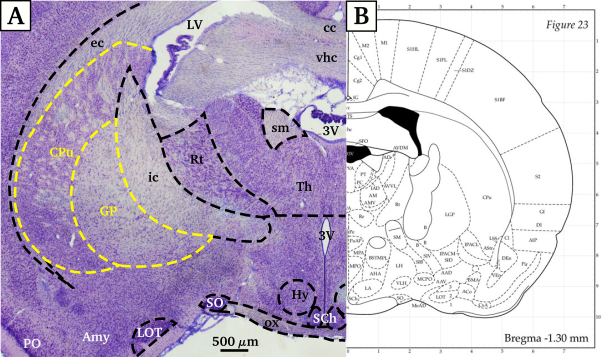
\includegraphics{pictures/Basalganglia/GP_CPu.png}
    \caption[Überblick Caudate putamen und Globus pallidus]{\textbf{Überblick Caudate putamen und Clobus pallidus.} \textbf{A:} Der Globus pallidus (GP) ist medial zum Caudate putamen (CPu) lokalisiert. Über die Fasern der Capsula interna (ic) wird er vom Thalamus (Th) abgerenzt. Weiter zeigt die Abbildung: dritter Ventrikel (3V), Amygdala (Amy), Corpus callosum (cc), Capsula externa (ec), Hypothalamus (Hy), Capsula interna (ic), lateraler Nucleus tractus olfactorius (LOT), lateraler Ventrikel (LV), Chiasma opticum (ox), primär olfaktorischer Cortex (PO),  Nucleus reticularis thalami (Rt), Nucleus suprachiasmicus (SCh), Stria medullaris thalami (sm), Nucleus supraopticus (SO), ventrale Hippocampuskommissur (vhc). Nissl-Färbung (N25~-~3). \textbf{B:} Dazugehörige Ansicht einer Schnittserie aus dem Rat Brain Atlas entnommen: \url{http://labs.gaidi.ca/rat-brain-atlas/}.}
    \label{fig:GP_CPu}
\end{figure}

\subsubsection*{Nucleus subthalamicus} \index{Nucleus! subthalamicus}
Der Ncl. subthalamicus ist ein Bestandteil des Subthalamus des Zwischenhirns. Es ist ein sehr kleines Kerngebiet, das zwischen dem Thalamus und der Substantia nigra lokalisiert ist (Abb.~\ref{fig:Nucleus_subthalamus}). Er erhält vorwiegend afferente Projektionen aus dem lateralen externen Pallidumsgebiet, aber auch aus dem Cortex, dem Hirnstamm und Thalamus. Die efferenten Fasern des Ncl. subthalamicus verlaufen zum medialen internen Pallidum und zur Substantia nigra pars reticulata. Über den Transmitter Glutamat wirken sie exzitatorisch auf diese Strukturen. Der Ncl. subthalamicus ist ein Bestandteil des indirekten Projektionswegs der Basalganglia. Über seine Aktivität kommt es zu einem hemmenden Ausgangssignal der Basalganglia, die eine bewegungsimpulshemmende Funktion ausübt\textsuperscript{\cite[Kap.~43]{kandel2013principles}, \cite[9]{trepel2011neuroanatomie}}.   

\begin{figure}[H]
    \centering
    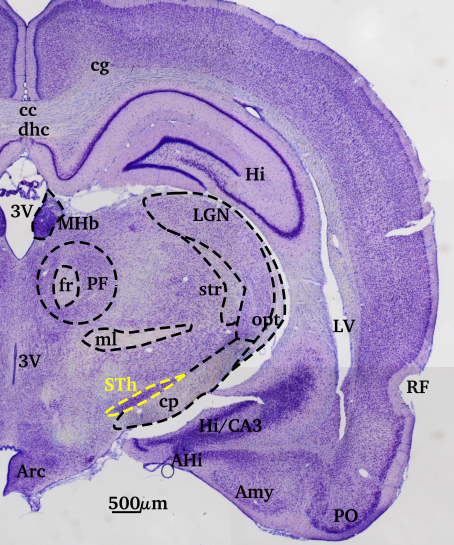
\includegraphics[width=0.7\textwidth]{pictures/Basalganglia/Nucleus_subthalamus.png}
    \caption[Nucleus subthalamicus]{\textbf{Nucleus subthalamicus.} Der Nucleus subthalamicus ist eine Struktur des Diencephalons, das sich ventro-lateral des Thalamus befindet. Nach außen wird es durch die Kleinhirnpedunkel (cp) eingegrenzt. Außerdem zeigt die Abbildung die Strukturen: dritter Ventrikel (3V), amygdaloid-hippocampale Area (AHi), Amygdala (Amy), Nucleus arcuatus hypothalami (Arc), Ammon's Horn (CA3), Corpus callosum (cc), Cingulum (cg), dorsale Hippocampuskomissur (dhc), Fasciculus retroflexus (fr), Hippocampus (Hi), Nucleus geniculatum laterale (LGN), lateraler Ventrikel (LV), Nucleus habenularis mediale (MHb), Leminiscus mediale (ml), optischer Tract (opt), Nucleus parafascicularis (PF),  primärer  olfaktorischer  Cortex (PO), Fissura rhinalis (RF), Nucleus subthalamicus (STh), Radiatio thalami superior (str). Nissl-Färbung (N20-4).}
    \label{fig:Nucleus_subthalamus}
\end{figure}

\subsubsection*{Substantia nigra} \index{Substantia nigra}
Die Substantia nigra ist ein Kerngebiet innerhalb das Mittelhirns, lokalisiert zwischen den Hirnschenkeln und dem Tegmentum (Abb.~\ref{fig:SN_Basalganglia}). Im Querschnitt weist dieses Kerngebiet eine starke schwarze Färbung auf, die durch den hohen Gehalt an Melanin in den Somata zustande kommt und der Region auch ihren Namen gibt. Weiter lässt sich die Substantia nigra in zwei Kerngebiete unterteilen, die \textbf{Pars compacta} und \textbf{Pars recticularis}. Diese beiden Bereiche unterscheiden sich in ihrem Aufbau, ihrer Funktion und ihren Faserverbindungen. Die Substantia nigra enthält zwei Typen von Neurone, die entweder Dopamin oder GABA als Neurotransmitter verwenden (Kap.~\ref{sec:transmittersysteme}). Dabei liegen die Zellkörper der dopaminergen Neurone vorwiegend in der Pars compacta und die GABAergen sind ausschließlich in der Pars reticularis zu finden. Die Substantia nigra pars reticularis fungiert als Ausgangsstruktur der Basalganglia und entspricht funktionell und anatomisch dem medialen Globus pallidus (s.o.). Die Pars compacta erhält neben den Afferenzen aus dem Striatum auch Input aus dem motorischen Gebieten des Großhirns. Die \textbf{Fribrae nigrostriatales} \index{Tractus! nigrostriatalis} stellen die primäre efferente Struktur dar. Die dopaminergen Fasern projizieren zum Striatum und wirken dort abhängig vom den dortigen dopaminergen Rezeptoren entweder hemmend oder erregend. Die hemmenden D1-Rezeptoren sind dabei auf der Gruppe dornentragenden Neurone zu finden, die direkt zu den Ausgangstrukturen der Basalganglia projizieren. Auf der zweiten Gruppe striataler Neurone, die den indirekten Projektionsweg nehmen, kommen die erregenden D2-Rezeptoren vor. Damit übernimmt die Substantia nigra pars compacta eine wichtige Funktion in der Modulation der direkten und indirekten Projektionswege durch die Basalganglia. Die Mehrheit der nigrostriatalen Fasern wirken jedoch hemmend auf das Striatum und vermitteln dadurch einen fördernden Einfluss auf die motorischen Impulse. Da die Substantia nigra auch durch das Striatum gehemmt wird, besteht eine negativ reziproke Rückkopplungsverbindung zwischen diesen beiden motorischen Zentren \textsuperscript{\cite[Kap.~17]{paxinos2014rat}, \cite[9]{trepel2011neuroanatomie}}.

\begin{figure}[H]
    \centering
    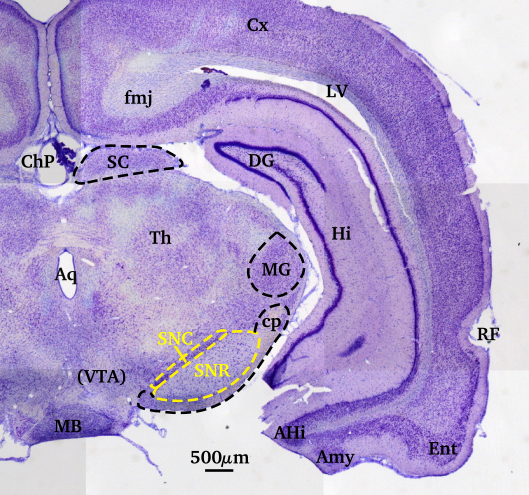
\includegraphics[width=\textwidth]{pictures/Basalganglia/SN.png}
    \caption[Substantia nigra]{\textbf{Substantia nigra.} Die Substantia nigra ist innerhalb des Mittelhirns zwischen dem Thalamus (Th) und den Hirnschenkeln lokalisiert. Sie besteht aus zwei Bereichen, der Pars compacta (SNC) und der Pars reticularis (SNR). Die Abbildung \textbf{A} (Nissel-Färbung: N18-4) zeigt auch:
    amygdaloid-hippocampale Area (AHi), Amygdala (Amy), Aquädukt (Aq), Plexus choroideus (ChP), Kleinhirnpedunkel (cp), Cortex (Cx), Gyrus dentatus (DG), Entorhinaler Cortex (Ent), Forceps major des Corpus callosum (fmj), Hippocampus (Hi), lateraler Ventrikel (LV), Mammillarkörper (MB), Nucleus geniculatum mediale (MGN), Fissura rhinalis (RF), Colliculus superior (SC), Area tegmentalis ventralis (VTA). Die Abbildung \textbf{B} (Ib09-4) zeigt die Substantia nigra im immunohistochemisch (Tyrosin-Hydroxilase-Nachweis) gefärbten Schnitt. Schnitt B liegt 600 $\upmu$m caudaler zu Schnitt A.}
    \label{fig:SN_Basalganglia}
\end{figure}

\subsubsection*{Direkte und indirekte Funktionsschleife durch die Basalganglia}
Das genaue Verschaltungsprinzip und Funktion der direkten und indirekten Projektionswege durch die Basalganglia wird hier genauer besprochen. Über die glutamatergen Fasern des Neocortex wird das Striatum erregt. Die dornentragenden Projektionsneurone des Striatums lassen sich dabei in zwei Gruppen unterteilen, die über zwei unterschiedliche Projektionswege eine funktionell antagonistisch Arbeitsweise der Basalganglia ermöglichen. Ein Teil der Neurone sendet Fasern zum lateralen Pallidum und die andere Hälfte zum medialen Pallidum und der Substantia nigra. Beide Gruppen haben eine hemmende Wirkung auf ihre Projektionsziele durch den Neurotranmitter GABA. Dennoch resultiert die Hemmung des medialen Pallidums und Substania nigra in einer erregenden, und die Inhibition des lateralen Segements in einer hemmenden Funktion auf motorische Impulse \textsuperscript{\cite[Kap.~9]{trepel2011neuroanatomie}}. \\  
\\ \noindent Beide Pallidumssegmente schütten GABA als Neurotransmitter aus und haben damit eine inhibitorische Wirkung. Das interne Pallidum, als Ausgangsstruktur der Basalganglia, projiziert inhibitorisch in den Ncl. ventralis anterolateralis des Thalamus. Die efferenten Fasern zu Motorkortex dieses Thalamuskern inhibieren normalerweise die motorischen Impulse. Wird die Interaktion des medialen Segments allerdings über die direkten Projektionsneurone des Striatums gehemmt, resultiert dies in einer erhöhten Thalamusaktivität, die auch an den motorischen Cortex weitergegeben wird. Dasselbe gilt auch für die Substantia nigra pars reticulata. Damit besteht die Funktion des direkten Projektionswegs der Basalganglia darin, ablaufende Bewegungen zu fördern durch eine positive Feedbackschleife. Der indirekten Projektionsweg auf der anderen Seite verläuft über den Ncl. subthalmicus. Die Hemmung des lateralen Palldiumssegement durch das Striatum führt zu einer Enthemmung des Ncl. subthalamicus. Dieser wiederum erregt den medialen Globus pallidus oder die Substantia nigra die daraufhin mit ihren inhibitorischen Projektionen die Aktivität der Thalamuskerne und des Cortex verringern. Somit lassen sich ungewollte Bewegungen unterdrücken (Abb.~\ref{fig:Verschaltung_Basalganglia}) \textsuperscript{\cite[Kap.~14]{crossman2014neuroanatomy}, \cite[9]{trepel2011neuroanatomie}}.\\ 
\\ \noindent Zusammenfassend lässt sich sagen, dass die erregenden motorischen Impulse aus dem Cortex über die Basalganglia auf zwei unterschiedliche Arten verschaltet werden kann. Dies resultiert dann entweder in einer inhibitorischen oder erregenden Regulation der ausgehenden motorischen Impulse der Basalganglia zurück zum Cortex. Die Funktion dabei besteht entweder in der Unterdrückung ungewollter Bewegungen oder in der Unterstützung gewollter und angepasster Bewegungen. Zudem wird davon ausgegangen, dass die beiden Projektionswege sich gegenseitig ausbalancieren und den Output der Basalganglia antagonistisch regulieren. Wenn sie im Ungleichgewicht sind entstehen daraus neurologische Störungen. Hypokinese, wie beispielsweise die Parkinson Erkrankung \index{Morbus Parkinson}, ist die Folge eines über-aktiven indirekten Projektionswegs. Das Gegenteil dazu die Hyperkinese bei Chorea Huntington \index{Chorea Huntington} Erkrankungen wird durch eine hohe Aktivität des direkten Wegs ausgelöst \textsuperscript{\cite[Kap.~17]{paxinos2014rat}}. 

\begin{figure}[H]
    \centering
    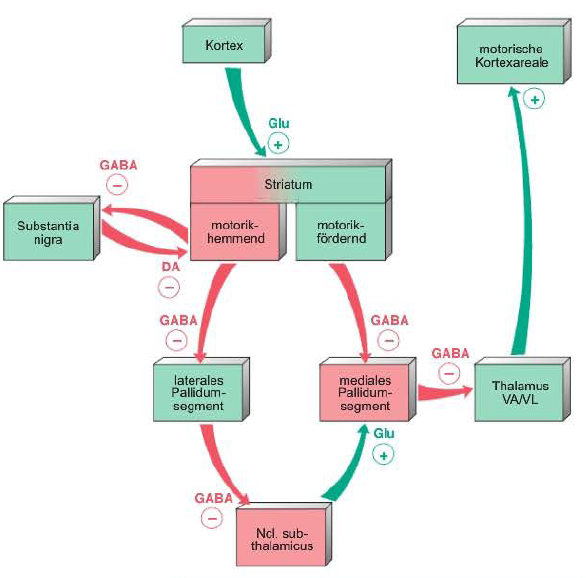
\includegraphics{pictures/Basalganglia/verschaltung_Basalganglien.PNG}
    \caption[Verschaltungsmuster der Basalganglia mit den beteiligten Transmittern]{\textbf{Verschaltungsmuster der Basalganglia mit den beteiligten Transmittern.} + (rot) bedeutet eine Erregung und - (grün)  steht für eine hemmende Projektion. Rot unterlegte Kästchen stellen ein motorikhemmendes, grün unterlegte ein motorikförderndes Zentrum dar. Abkürzungen: DA = Dopamin, GABA = y-Aminobuttersäure, Glu = Glutamat. VA/VL = Ncl. ventralis anterolateralis des Thalamus. \\ Abbildung aus \textit{Neuroanatomie}, Trepel \textsuperscript{\cite[Kap.~9]{trepel2011neuroanatomie}}.}
    \label{fig:Verschaltung_Basalganglia}
\end{figure}

